\documentclass[12pt]{article}
\usepackage[utf8]{inputenc}
\usepackage[T1]{fontenc}
\usepackage[french]{babel}
\usepackage{graphicx}
\usepackage[top=3cm,bottom=2.5cm,left=2.5cm,right=2.5cm]{geometry}

\renewcommand{\contentsname}{Sommaire}
\renewcommand{\thesection}{\Roman{section} -~}
\renewcommand{\thesubsection}{\Alph{subsection})}

\newcommand{\Octave}{GNU Octave }
\newcommand{\Matlab}{MATLAB\textsuperscript{\textregistered} }

\title{License SPI -- Projet Auralisation}
\author{Thomas \textsc{Lechat} \and Xin \textsc{Wang} \and Mathieu \textsc{Gaborit}}
\date{Note de synthèse 5 -- Décembre 2012}


\begin{document}

\maketitle

Pendant cette séance nous nous sommes encore une fois séparés en 2 groupes afin de réaliser le maximum de mesures différentes. Le but est de prendre une mesure de reponse impulsionnelle ainsi que de 3 sons différents dans une salle de TP afin de pouvoir comparer ces sons avec ceux d'une salle reverbérante. Ainsi nous pourrons ainsi comparer l'auralisation de 2 salles et donc voir dans quel mesure le procédé d'auralisation permet un rendu précis des caractéristiques de la salle auralisé.

\section{Mesures dans une salle de TP} % {{{1
Nous avons effectué pendant cette séance une serie de mesure dans le salle de TP Mersenne et ce pour différentes positions de la source ainsi que du recepteur (et de leur orientation l'un par rapport à l'autre). 

Les reponses impulsionnelles ont été prises à l'aide d'un ballon pour différentes positions des récepteurs dans la salle, de plus la tête artificielle a été utilisée afin d'avoir les reponses monaurales et binaurales.  

Enfin la reponse impulsionnelle binaurale a été prise pour différentes orientations de la tête vis à vis de la source la source afin de pouvoir determiner si oui où non la réponse impulsionnelle suffisait pour situer le son dans l'espace.

\section{Caractérisation de la chaîne d'excitation électro-acoustique} % {{{1

Une mesure de la reponse en fréquence de la chaîne d'excitation a été effectuée pour savoir dans quelle mesure celle-ci influe sur notre signal d'excitation. L'objectif est de pouvoir à terme comparer des RI prises avec une source electro-acoustique et des RI prises avec un ballon. Le  schéma du montage pour la mesure de la réponse en fréquence de la source est visible en figure~\ref{carac_source}.

\begin{figure}[h!]
\begin{center}
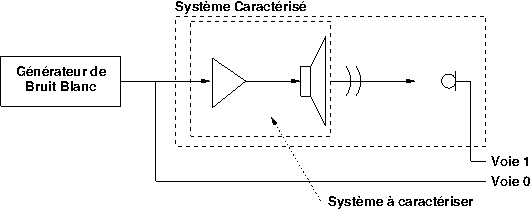
\includegraphics[width=10cm]{carac_source}
\end{center}
\caption{\label{carac_source}Schéma du montage utilisé pour caractériser la source, le tout étant placé dans un caisson anéchoïque. A noter la différence entre le système à caractériser et le système réellement caractérisé.}
\end{figure}

La mesure a été effectuée dans un caisson anéchoïque (caisse dont les parois sont tapissées de mousse), le haut parleur étant placé au fond de celui ci et le microphone à l'opposé de celui ci.

Le but est d'en déduire la reponse en fréquence de la chaîne d'excitation et ainsi la prendre en compte lors de l'auralisation.

Ayant mesuré et calculé la réponse en fréquence de la source électro-acoustique, nous devrions être en mesure de compenser une parties des erreurs liées à son utilisation.


\section{Analyse des données} % {{{1

\subsection{Bug d'\emph{Analyseur CTTM}}% {{{2

Au cours de l'analyse des données et du traitement des signaux mesurés il est apparu que le logiciel \emph{Analyseur CTTM} n'utilisaits la fréquence d'échantillonnage qu'il affichait... Travaillant principalement dans la bande audio (et pour des applications audio), nous utilisions jusqu'alors une fréquence d'échantillonnage de 44100Hz. Après reconstruction d'un fichier audio à partir de données mesurées et stockées en \textit{plain text}, nous avons noté que le signal (une musique) était plus grave et lente que d'habitude mais que ce n'était pas le cas sur les fichiers audio directement générés par \emph{Analyseur CTTM}. Quelques vérification plus tard, il était clair que même s'il était réglé pour enregistrer en échantillonnant à 44100Hz, il ne prenait pas en compte cette valeur et travaillait à 51200Hz. Nous envisageons de faire remonter le bug.

Afin d'accélérer le processus de convolution (un script par paire {son,RI}), nous avons écrit un script "type" prenant une liste de sons anéchoïques, d'enregistrements de référence et une RI en entrée et qui crée en sortie un fichier pour chaque convolution et un WAV contenant le fichier audio de référence recréé à partir des mesures en TXT.

\subsection{Ecoute des convolutions et comparaison perceptuelle} % {{{2

Après avoir fait plusieurs essais de convolution, nous avons écouté les résultats et les avons comparé perceptuellement aux signaux «de référence». Les signaux «de référence» sont les mêmes sont anéchoïques que ceux utilisés dans la convolution joués dans la salle cible.

Nous avons notés que le RSB des mesures «de référence» était assez faible, de plus le niveau global inscrit dans les fichier TXT est très faible, il faudra peut être y remédier. A noter aussi les bruits parasites au début des bandes de signaux convolués. Ceux ci peuvent être liés au fait que les bandes de RI n'aient pas été recoupées avant convolution pour «coller» au plus proche de la RI.

Ces deux points constituent les objectifs de la prochaine séance en terme de traitement du signal.

On cherchera aussi à améliorer le script de convolution «à la chaine».

% }}}
\end{document}
